% Options for packages loaded elsewhere
% Options for packages loaded elsewhere
\PassOptionsToPackage{unicode}{hyperref}
\PassOptionsToPackage{hyphens}{url}
\PassOptionsToPackage{dvipsnames,svgnames,x11names}{xcolor}
%
\documentclass[
  letterpaper,
  DIV=11,
  numbers=noendperiod]{scrartcl}
\usepackage{xcolor}
\usepackage{amsmath,amssymb}
\setcounter{secnumdepth}{5}
\usepackage{iftex}
\ifPDFTeX
  \usepackage[T1]{fontenc}
  \usepackage[utf8]{inputenc}
  \usepackage{textcomp} % provide euro and other symbols
\else % if luatex or xetex
  \usepackage{unicode-math} % this also loads fontspec
  \defaultfontfeatures{Scale=MatchLowercase}
  \defaultfontfeatures[\rmfamily]{Ligatures=TeX,Scale=1}
\fi
\usepackage{lmodern}
\ifPDFTeX\else
  % xetex/luatex font selection
\fi
% Use upquote if available, for straight quotes in verbatim environments
\IfFileExists{upquote.sty}{\usepackage{upquote}}{}
\IfFileExists{microtype.sty}{% use microtype if available
  \usepackage[]{microtype}
  \UseMicrotypeSet[protrusion]{basicmath} % disable protrusion for tt fonts
}{}
\makeatletter
\@ifundefined{KOMAClassName}{% if non-KOMA class
  \IfFileExists{parskip.sty}{%
    \usepackage{parskip}
  }{% else
    \setlength{\parindent}{0pt}
    \setlength{\parskip}{6pt plus 2pt minus 1pt}}
}{% if KOMA class
  \KOMAoptions{parskip=half}}
\makeatother
% Make \paragraph and \subparagraph free-standing
\makeatletter
\ifx\paragraph\undefined\else
  \let\oldparagraph\paragraph
  \renewcommand{\paragraph}{
    \@ifstar
      \xxxParagraphStar
      \xxxParagraphNoStar
  }
  \newcommand{\xxxParagraphStar}[1]{\oldparagraph*{#1}\mbox{}}
  \newcommand{\xxxParagraphNoStar}[1]{\oldparagraph{#1}\mbox{}}
\fi
\ifx\subparagraph\undefined\else
  \let\oldsubparagraph\subparagraph
  \renewcommand{\subparagraph}{
    \@ifstar
      \xxxSubParagraphStar
      \xxxSubParagraphNoStar
  }
  \newcommand{\xxxSubParagraphStar}[1]{\oldsubparagraph*{#1}\mbox{}}
  \newcommand{\xxxSubParagraphNoStar}[1]{\oldsubparagraph{#1}\mbox{}}
\fi
\makeatother


\usepackage{longtable,booktabs,array}
\newcounter{none} % for unnumbered tables
\usepackage{calc} % for calculating minipage widths
% Correct order of tables after \paragraph or \subparagraph
\usepackage{etoolbox}
\makeatletter
\patchcmd\longtable{\par}{\if@noskipsec\mbox{}\fi\par}{}{}
\makeatother
% Allow footnotes in longtable head/foot
\IfFileExists{footnotehyper.sty}{\usepackage{footnotehyper}}{\usepackage{footnote}}
\makesavenoteenv{longtable}
\usepackage{graphicx}
\makeatletter
\newsavebox\pandoc@box
\newcommand*\pandocbounded[1]{% scales image to fit in text height/width
  \sbox\pandoc@box{#1}%
  \Gscale@div\@tempa{\textheight}{\dimexpr\ht\pandoc@box+\dp\pandoc@box\relax}%
  \Gscale@div\@tempb{\linewidth}{\wd\pandoc@box}%
  \ifdim\@tempb\p@<\@tempa\p@\let\@tempa\@tempb\fi% select the smaller of both
  \ifdim\@tempa\p@<\p@\scalebox{\@tempa}{\usebox\pandoc@box}%
  \else\usebox{\pandoc@box}%
  \fi%
}
% Set default figure placement to htbp
\def\fps@figure{htbp}
\makeatother


% definitions for citeproc citations
\NewDocumentCommand\citeproctext{}{}
\NewDocumentCommand\citeproc{mm}{%
  \begingroup\def\citeproctext{#2}\cite{#1}\endgroup}
\makeatletter
 % allow citations to break across lines
 \let\@cite@ofmt\@firstofone
 % avoid brackets around text for \cite:
 \def\@biblabel#1{}
 \def\@cite#1#2{{#1\if@tempswa , #2\fi}}
\makeatother
\newlength{\cslhangindent}
\setlength{\cslhangindent}{1.5em}
\newlength{\csllabelwidth}
\setlength{\csllabelwidth}{3em}
\newenvironment{CSLReferences}[2] % #1 hanging-indent, #2 entry-spacing
 {\begin{list}{}{%
  \setlength{\itemindent}{0pt}
  \setlength{\leftmargin}{0pt}
  \setlength{\parsep}{0pt}
  % turn on hanging indent if param 1 is 1
  \ifodd #1
   \setlength{\leftmargin}{\cslhangindent}
   \setlength{\itemindent}{-1\cslhangindent}
  \fi
  % set entry spacing
  \setlength{\itemsep}{#2\baselineskip}}}
 {\end{list}}
\usepackage{calc}
\newcommand{\CSLBlock}[1]{\hfill\break\parbox[t]{\linewidth}{\strut\ignorespaces#1\strut}}
\newcommand{\CSLLeftMargin}[1]{\parbox[t]{\csllabelwidth}{\strut#1\strut}}
\newcommand{\CSLRightInline}[1]{\parbox[t]{\linewidth - \csllabelwidth}{\strut#1\strut}}
\newcommand{\CSLIndent}[1]{\hspace{\cslhangindent}#1}



\setlength{\emergencystretch}{3em} % prevent overfull lines

\providecommand{\tightlist}{%
  \setlength{\itemsep}{0pt}\setlength{\parskip}{0pt}}



 


\KOMAoption{captions}{tableheading}
\makeatletter
\@ifpackageloaded{caption}{}{\usepackage{caption}}
\AtBeginDocument{%
\ifdefined\contentsname
  \renewcommand*\contentsname{Table of contents}
\else
  \newcommand\contentsname{Table of contents}
\fi
\ifdefined\listfigurename
  \renewcommand*\listfigurename{List of Figures}
\else
  \newcommand\listfigurename{List of Figures}
\fi
\ifdefined\listtablename
  \renewcommand*\listtablename{List of Tables}
\else
  \newcommand\listtablename{List of Tables}
\fi
\ifdefined\figurename
  \renewcommand*\figurename{Figure}
\else
  \newcommand\figurename{Figure}
\fi
\ifdefined\tablename
  \renewcommand*\tablename{Table}
\else
  \newcommand\tablename{Table}
\fi
}
\@ifpackageloaded{float}{}{\usepackage{float}}
\floatstyle{ruled}
\@ifundefined{c@chapter}{\newfloat{codelisting}{h}{lop}}{\newfloat{codelisting}{h}{lop}[chapter]}
\floatname{codelisting}{Listing}
\newcommand*\listoflistings{\listof{codelisting}{List of Listings}}
\makeatother
\makeatletter
\makeatother
\makeatletter
\@ifpackageloaded{caption}{}{\usepackage{caption}}
\@ifpackageloaded{subcaption}{}{\usepackage{subcaption}}
\makeatother
\usepackage{bookmark}
\IfFileExists{xurl.sty}{\usepackage{xurl}}{} % add URL line breaks if available
\urlstyle{same}
\hypersetup{
  pdftitle={We Are Different And We Are Similar},
  pdfauthor={Andy Grogan-Kaylor},
  colorlinks=true,
  linkcolor={blue},
  filecolor={Maroon},
  citecolor={Blue},
  urlcolor={Blue},
  pdfcreator={LaTeX via pandoc}}


\title{We Are Different And We Are Similar}
\usepackage{etoolbox}
\makeatletter
\providecommand{\subtitle}[1]{% add subtitle to \maketitle
  \apptocmd{\@title}{\par {\large #1 \par}}{}{}
}
\makeatother
\subtitle{Universals, Commonality, Diversity and Variation In Parenting
and Child Development}
\author{Andy Grogan-Kaylor}
\date{2026-04-07}
\begin{document}
\maketitle

\renewcommand*\contentsname{Table of contents}
{
\setcounter{tocdepth}{3}
\tableofcontents
}

\section{Acknowledgements}\label{acknowledgements}

\begin{itemize}
\tightlist
\item
  Collaborators:

  \begin{itemize}
  \tightlist
  \item
    Professor Julie Ma
  \item
    Professor Yoonsun Han
  \item
    Dr.~Kaitlin Ward
  \end{itemize}
\item
  Members of the \emph{Global Families Project}
\item
  IPUMS
\item
  NICHD
\end{itemize}

\section{The Big Ideas}\label{the-big-ideas}

\subsection{The Scope of the Issue}\label{the-scope-of-the-issue}

\begin{itemize}
\tightlist
\item
  UNICEF considers children globally to be in {crisis}: political
  violence, climate change, and poverty affect many children (UNICEF,
  2024a, 2024b).
\item
  In this time of crisis, {parenting} is one crucial area of focus.
\item
  According to UNICEF data, {\(\frac{1}{3}\) of children are subject to
  physical punishment} (Ward et al., 2023); {\(\frac{2}{3}\) to some
  form of violent punishment} (UNICEF, 2024a).
\item
  In a review of 50 years of literature on physical punishment, Gershoff
  \& Grogan-Kaylor (2016) {connect physical punishment to poor mental
  health outcomes}, and other poor outcomes over the life course. Ward
  et al. (2023) examines the {relationship of multiple forms of parental
  discipline to child outcomes}.
\end{itemize}

\subsection{Are We Similar? Are We
Different?}\label{are-we-similar-are-we-different}

\begin{figure}

\begin{minipage}[t]{0.50\linewidth}

\begin{figure}[H]

{\centering \pandocbounded{\includegraphics[keepaspectratio]{positiveparenting.png}}

}

\subcaption{positive parenting}

\end{figure}%

\end{minipage}%
%
\begin{minipage}[t]{0.50\linewidth}

\begin{figure}[H]

{\centering \pandocbounded{
\includegraphics[keepaspectratio]{MICS.png}}

}

\subcaption{countries in MICS data}

\end{figure}%

\end{minipage}%

\end{figure}%

\subsection{Both Universals and Variation Are
Important}\label{both-universals-and-variation-are-important}

\begin{quote}
``Despite the {incredible diversity} existing among and within human
cultures, there are many phenomena that occur regularly in all known
societies. These {commonalities, or universals}, while deriving in part
from human nature, may also have specific social, cultural, and systemic
sources. We need to develop a working understanding of these universals
so that we might advance legitimate, empirically based human science set
on creating knowledge that is politically relevant to {fostering real
solutions} to the problems that complicate human co-existence in the Age
of the Anthropocene.'' (Antweiler, 2016)
\end{quote}

\subsection{Highlighting Commonalities May Promote Intergroup Attitudes
And
Solidarity}\label{highlighting-commonalities-may-promote-intergroup-attitudes-and-solidarity}

\begin{quote}
``Hanel et al. (2019) cite research suggesting that `highlighting
similarities between groups {improves interpersonal and intergroup
attitudes}.' Others have argued that `build{[}ing{]} bonds of
commonality across our differences' might be an {impetus for social
transformation} (Hunt-Hendrix \& Taylor, 2024).''
\end{quote}

\subsection{The Argument Of This
Presentation}\label{the-argument-of-this-presentation}

\begin{itemize}
\tightlist
\item
  Families, parents and children experience an incredible {diversity of
  circumstances}.
\item
  Parents engage in {parenting behaviors} with consequent diversity,
  though with some surprising similarities.
\item
  The {associations} of parenting with child outcomes are surprisingly
  consistent.
\end{itemize}

\section{The Study}\label{the-study}

\subsection{Data}\label{data}

MICS data collected by UNICEF from Low and Middle Income Countries
(LMIC) around the world.
\(N = 224,632 \text{ families}; N_{countries} = 60\)

Contains questions about {parental discipline (both positive and
negative)} and {child aggression} .

\begin{verbatim}
Error in `value[[3L]]()`:
! Failed to install the rnaturalearthdata package. Please try installing
  the package for yourself using the following command:
  `install.packages("rnaturalearthdata")`
\end{verbatim}

\begin{verbatim}
Error:
! object 'mapdata' not found
\end{verbatim}

\begin{figure}[H]

{\centering \pandocbounded{
\includegraphics[keepaspectratio]{MICS.png}}

}

\caption{countries in UNICEF MICS Data}

\end{figure}%

\subsection{Sources of Variation In The Study of Parenting And Child
Outcomes}\label{sources-of-variation-in-the-study-of-parenting-and-child-outcomes}

\begin{figure}

\centering{

\pandocbounded{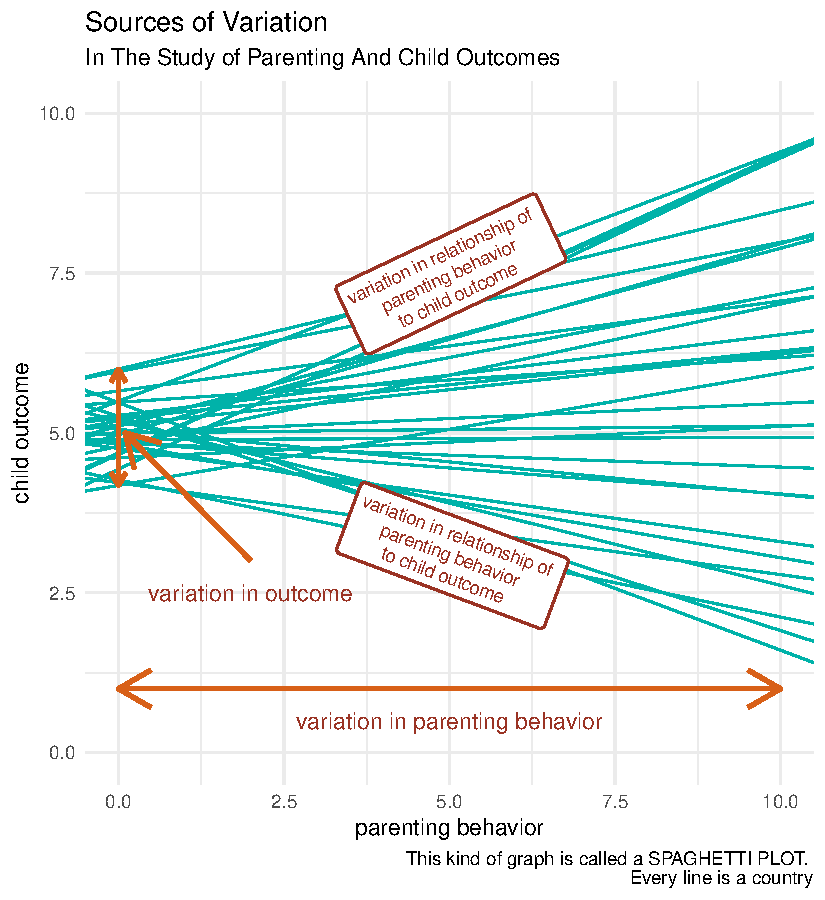
\includegraphics[keepaspectratio]{positive-and-negative-parenting_files/figure-pdf/fig-variationsources-1.pdf}}

}

\caption{\label{fig-variationsources}Sources of Variation In The Study
of Parenting And Child Outcomes}

\end{figure}%

\subsection{Check-In}\label{check-in}

Are we OK? Are there questions?

\subsection{Sources of Variation (2)}\label{sources-of-variation-2}

\begin{figure}[H]

{\centering 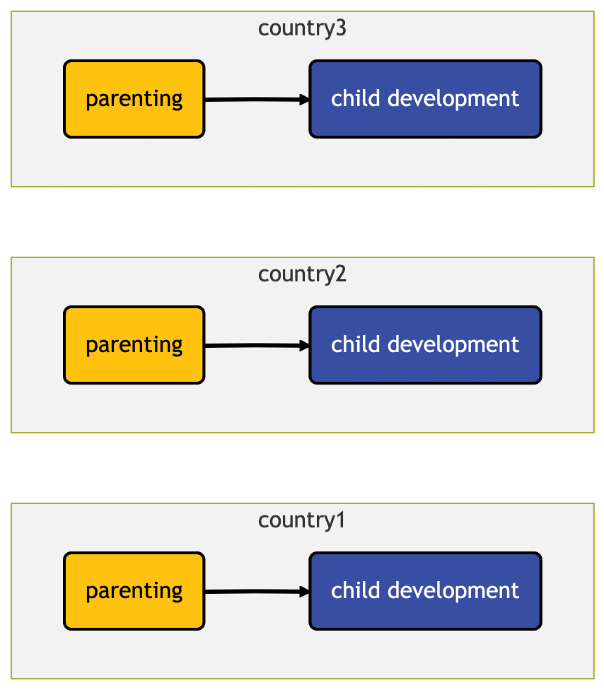
\includegraphics[width=0.5\linewidth,height=\textheight,keepaspectratio]{visual-question-diagram.png}

}

\caption{a visual version of the research question}

\end{figure}%

\subsection{The Equation}\label{the-equation}

\begin{figure}[H]

{\centering \pandocbounded{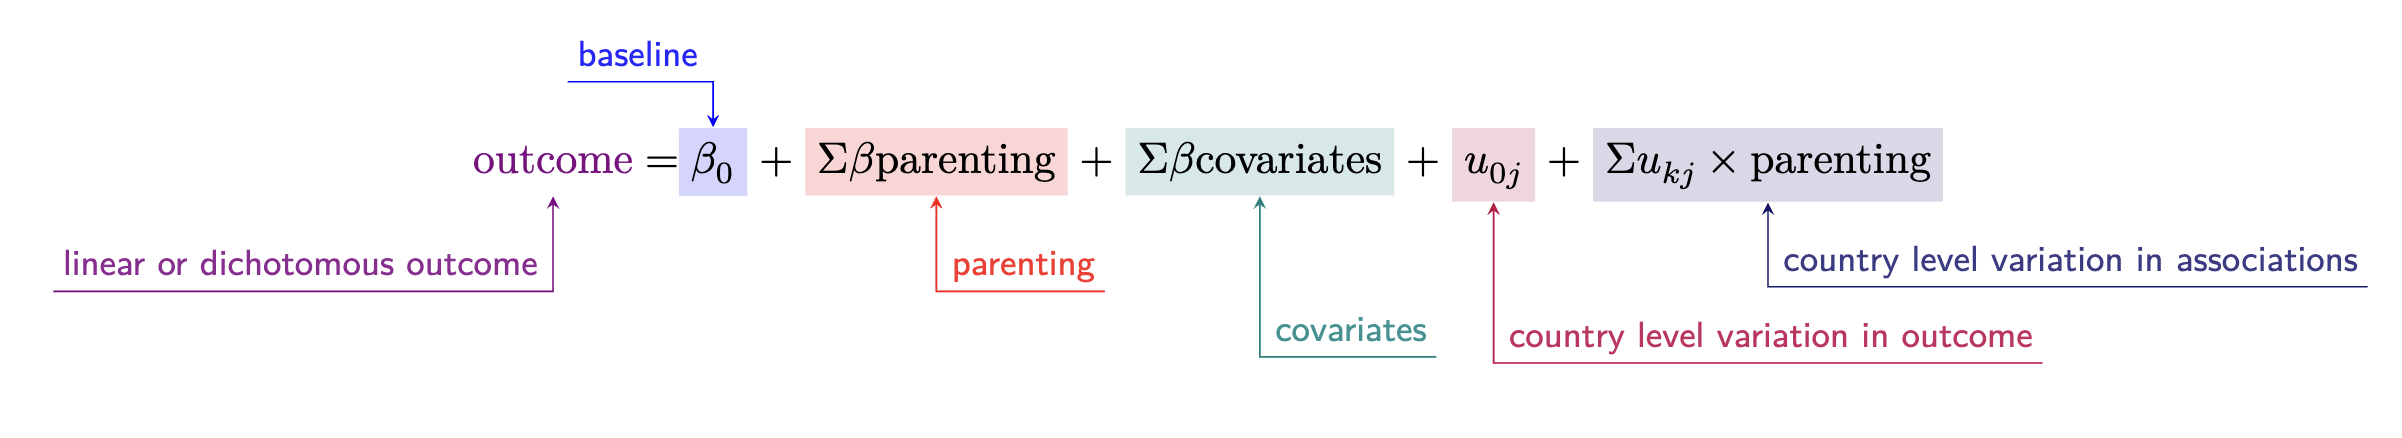
\includegraphics[keepaspectratio]{annotated-equation.png}}

}

\caption{annotated equation}

\end{figure}%

\subsection{\texorpdfstring{Parenting Behaviors Vary \emph{Somewhat}
Across
Countries}{Parenting Behaviors Vary Somewhat Across Countries}}\label{parenting-behaviors-vary-somewhat-across-countries}

\emph{Verbal reasoning} and \emph{shouting} are the most common parental
discipline behaviors toward young children.

\begin{figure}[H]

{\centering \pandocbounded{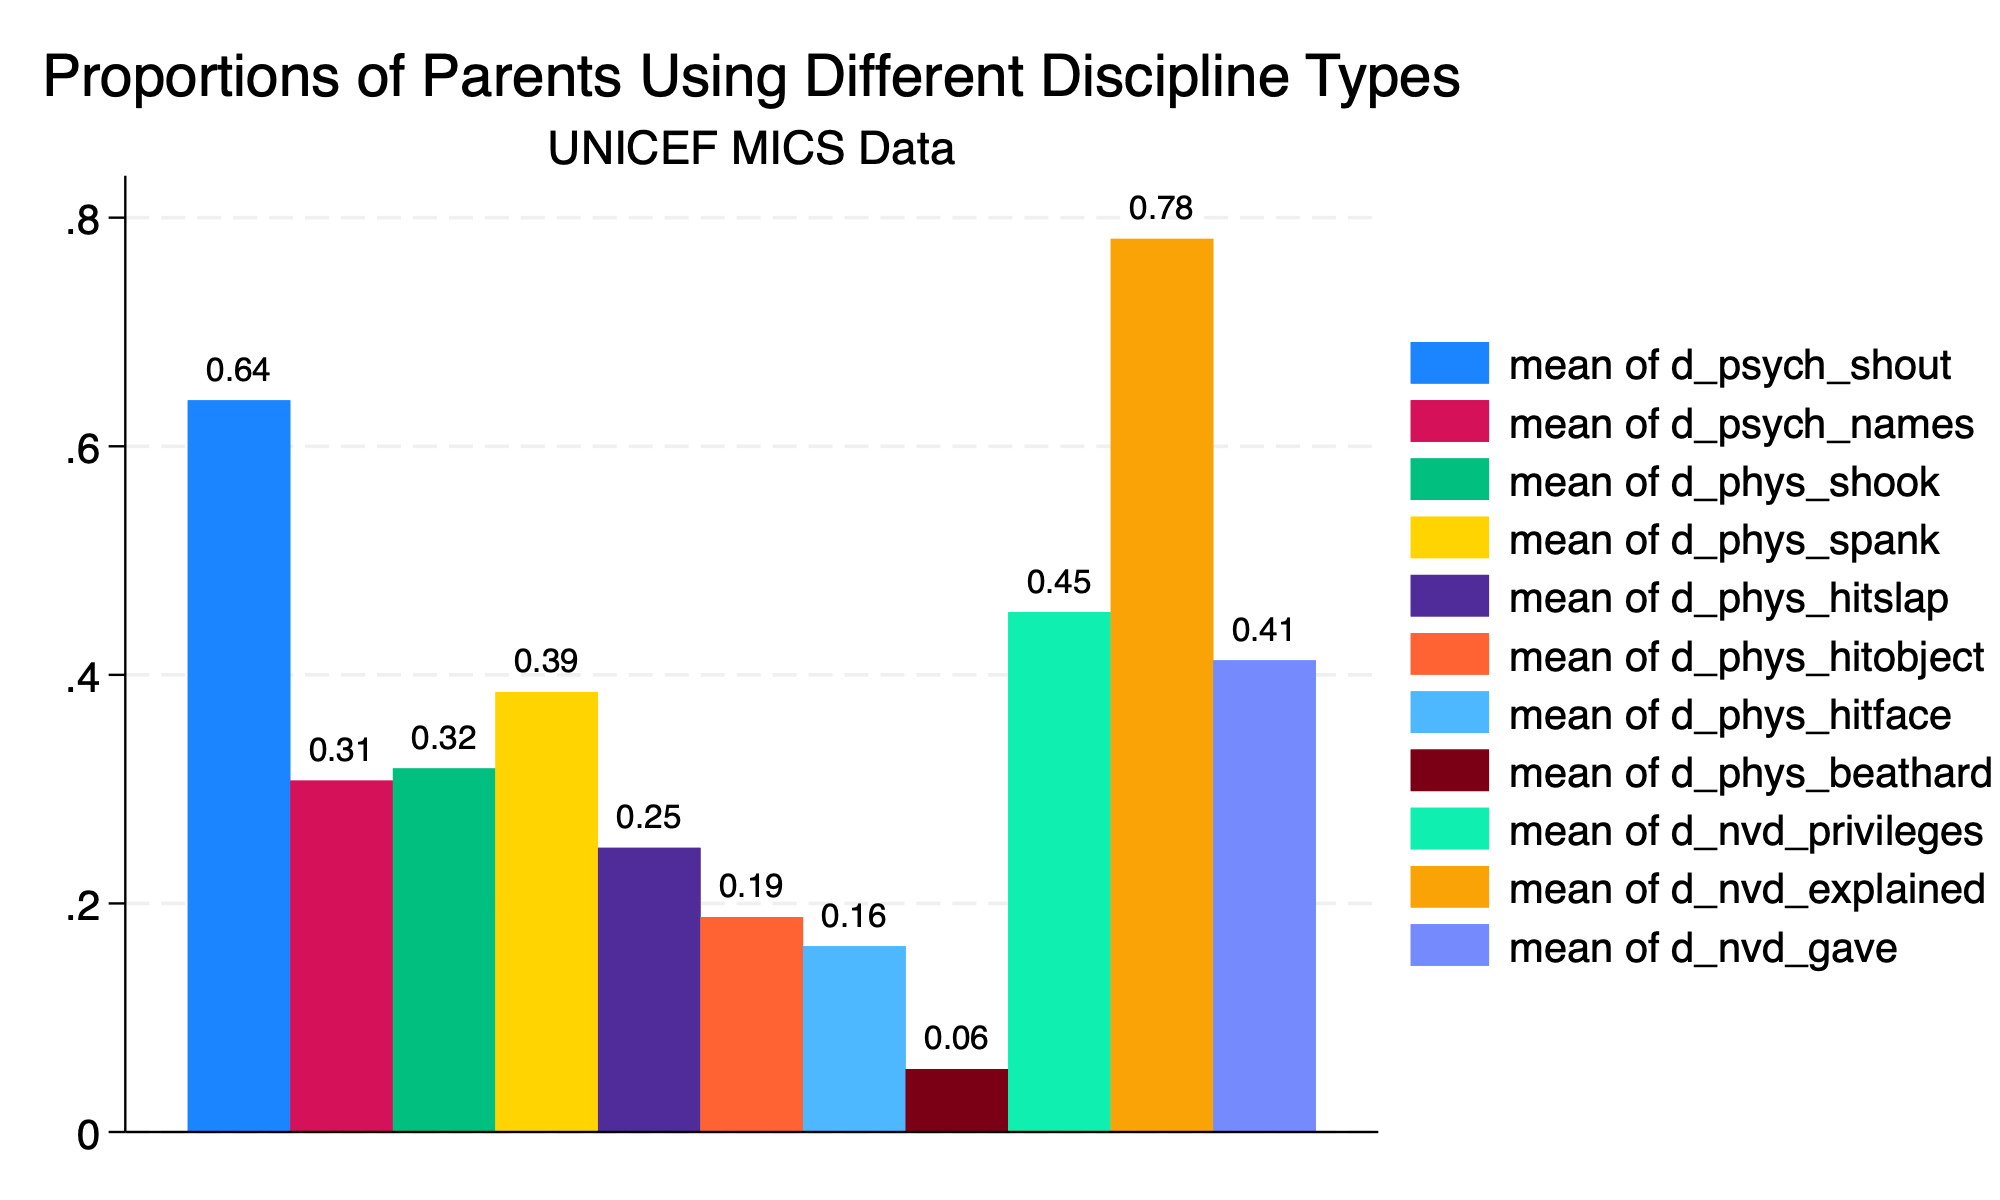
\includegraphics[keepaspectratio]{descriptives.png}}

}

\caption{positive and negative parenting}

\end{figure}%

\subsection{\texorpdfstring{The \emph{Maximal Model}
Approach}{The Maximal Model Approach}}\label{the-maximal-model-approach}

\begin{itemize}
\tightlist
\item
  Hypothetically, one might imagine that there could be group level
  {unobserved factors which affect many regression slopes}--i.e.~the
  relationship between multiple predictors (e.g.~\(x_1\), \(x_2\),
  \(x_3\), etc.) and outcome variable \(y\).
\item
  Arguably, were one to ignore these unobserved factors in statistical
  estimation, they would show up either in an error term (\(e_i\) or
  \(u_0\)), or in the regression coefficients (\(\beta\)). This could be
  seen as a form of {statistical bias}.
\item
  The above could lead to a {substantive mis-estimation of important
  effects}. Thus, there is a conceptual argument for including as many
  random effects---i.e.~random slopes---in a statistical model as
  possible (Barr et al., 2013; Frank, 2018).
\item
  There is also a substantive reason: {We might be interested in the
  \emph{variation} of \emph{all} the random slopes!}
\end{itemize}

\begin{figure}[H]

{\centering \pandocbounded{
\includegraphics[keepaspectratio]{variationsources.png}}

}

\caption{sources of variation}

\end{figure}%

\subsection{Relationship of Parenting And Child
Outcomes}\label{relationship-of-parenting-and-child-outcomes}

Maximal Model of Parenting and Child Aggression Outcome

{\def\LTcaptype{none} % do not increment counter
\begin{longtable}[]{@{}lll@{}}
\toprule\noalign{}
& aggress & \\
\midrule\noalign{}
\endhead
\bottomrule\noalign{}
\endlastfoot
child aggression & & \\
Sex of randomly selected child & -0.023 & ** \\
Age of randomly selected child & 0.000 & \\
Selected child shouted at & 0.036 & ** \\
Selected child called dumb/lazy/names & 0.054 & ** \\
Selected child shaken & 0.039 & ** \\
Selected child spanked & 0.023 & ** \\
Selected child hit/slapped on hand/arm/leg & 0.033 & ** \\
Selected child hit with belt/brush/stick/etc & 0.035 & ** \\
Selected child hit/slapped on face/head/ears & 0.044 & ** \\
Selected child beat as hard as one could & 0.026 & ** \\
Selected child's privileges taken away & 0.007 & \\
Selected child - explained why behavior wrong & -0.014 & * \\
Selected child given something else to do & 0.004 & \\
Intercept & 0.325 & ** \\
country & & \\
var(d\_psych\_shout) & 0.001 & \\
var(d\_psych\_names) & 0.001 & \\
var(d\_phys\_shook) & 0.001 & \\
var(d\_phys\_spank) & 0.001 & \\
var(d\_phys\_hitslap) & 0.001 & \\
var(d\_phys\_hitobject) & 0.001 & \\
var(d\_phys\_hitface) & 0.002 & \\
var(d\_phys\_beathard) & 0.002 & \\
var(d\_nvd\_privileges) & 0.001 & \\
var(d\_nvd\_explained) & 0.001 & \\
var(d\_nvd\_gave) & 0.001 & \\
var(\_cons) & 0.012 & \\
Residual & & \\
var(e) & 0.217 & \\
Number of observations & 224632 & \\
\end{longtable}
}

** p\textless.01, * p\textless.05

\section{The Relationship of Parenting And Child Outcomes Shows Little
Variation Across
Countries}\label{the-relationship-of-parenting-and-child-outcomes-shows-little-variation-across-countries}

\subsection{A Standard Spaghetti Plot}\label{a-standard-spaghetti-plot}

\begin{figure}[H]

{\centering \pandocbounded{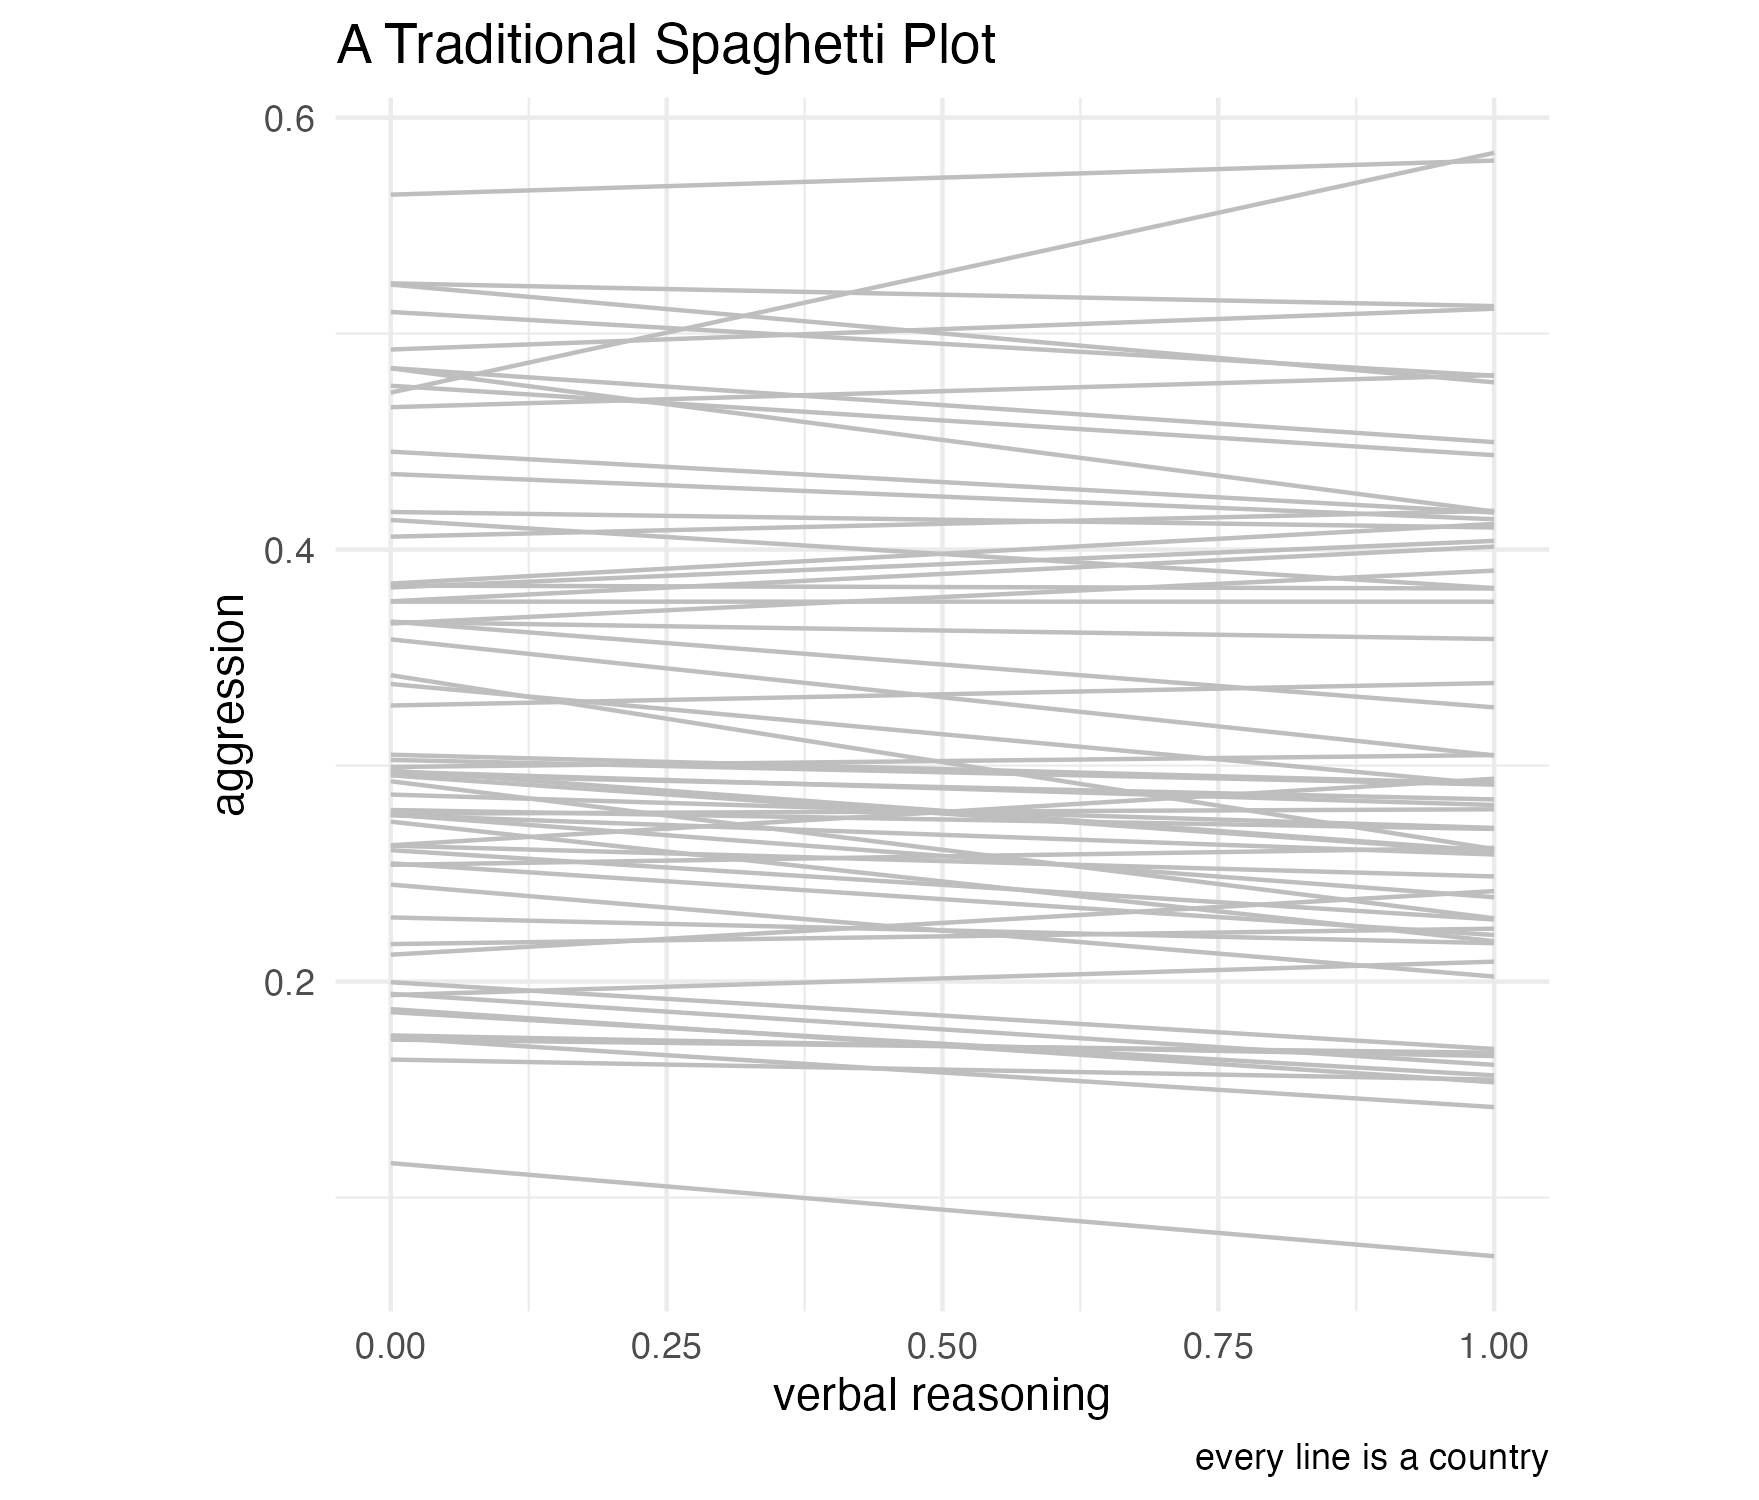
\includegraphics[keepaspectratio]{explain-spaghetti-plot0.png}}

}

\caption{a standard `spaghetti' plot}

\end{figure}%

\subsection{A Modified Spaghetti Plot}\label{a-modified-spaghetti-plot}

\begin{figure}[H]

{\centering \pandocbounded{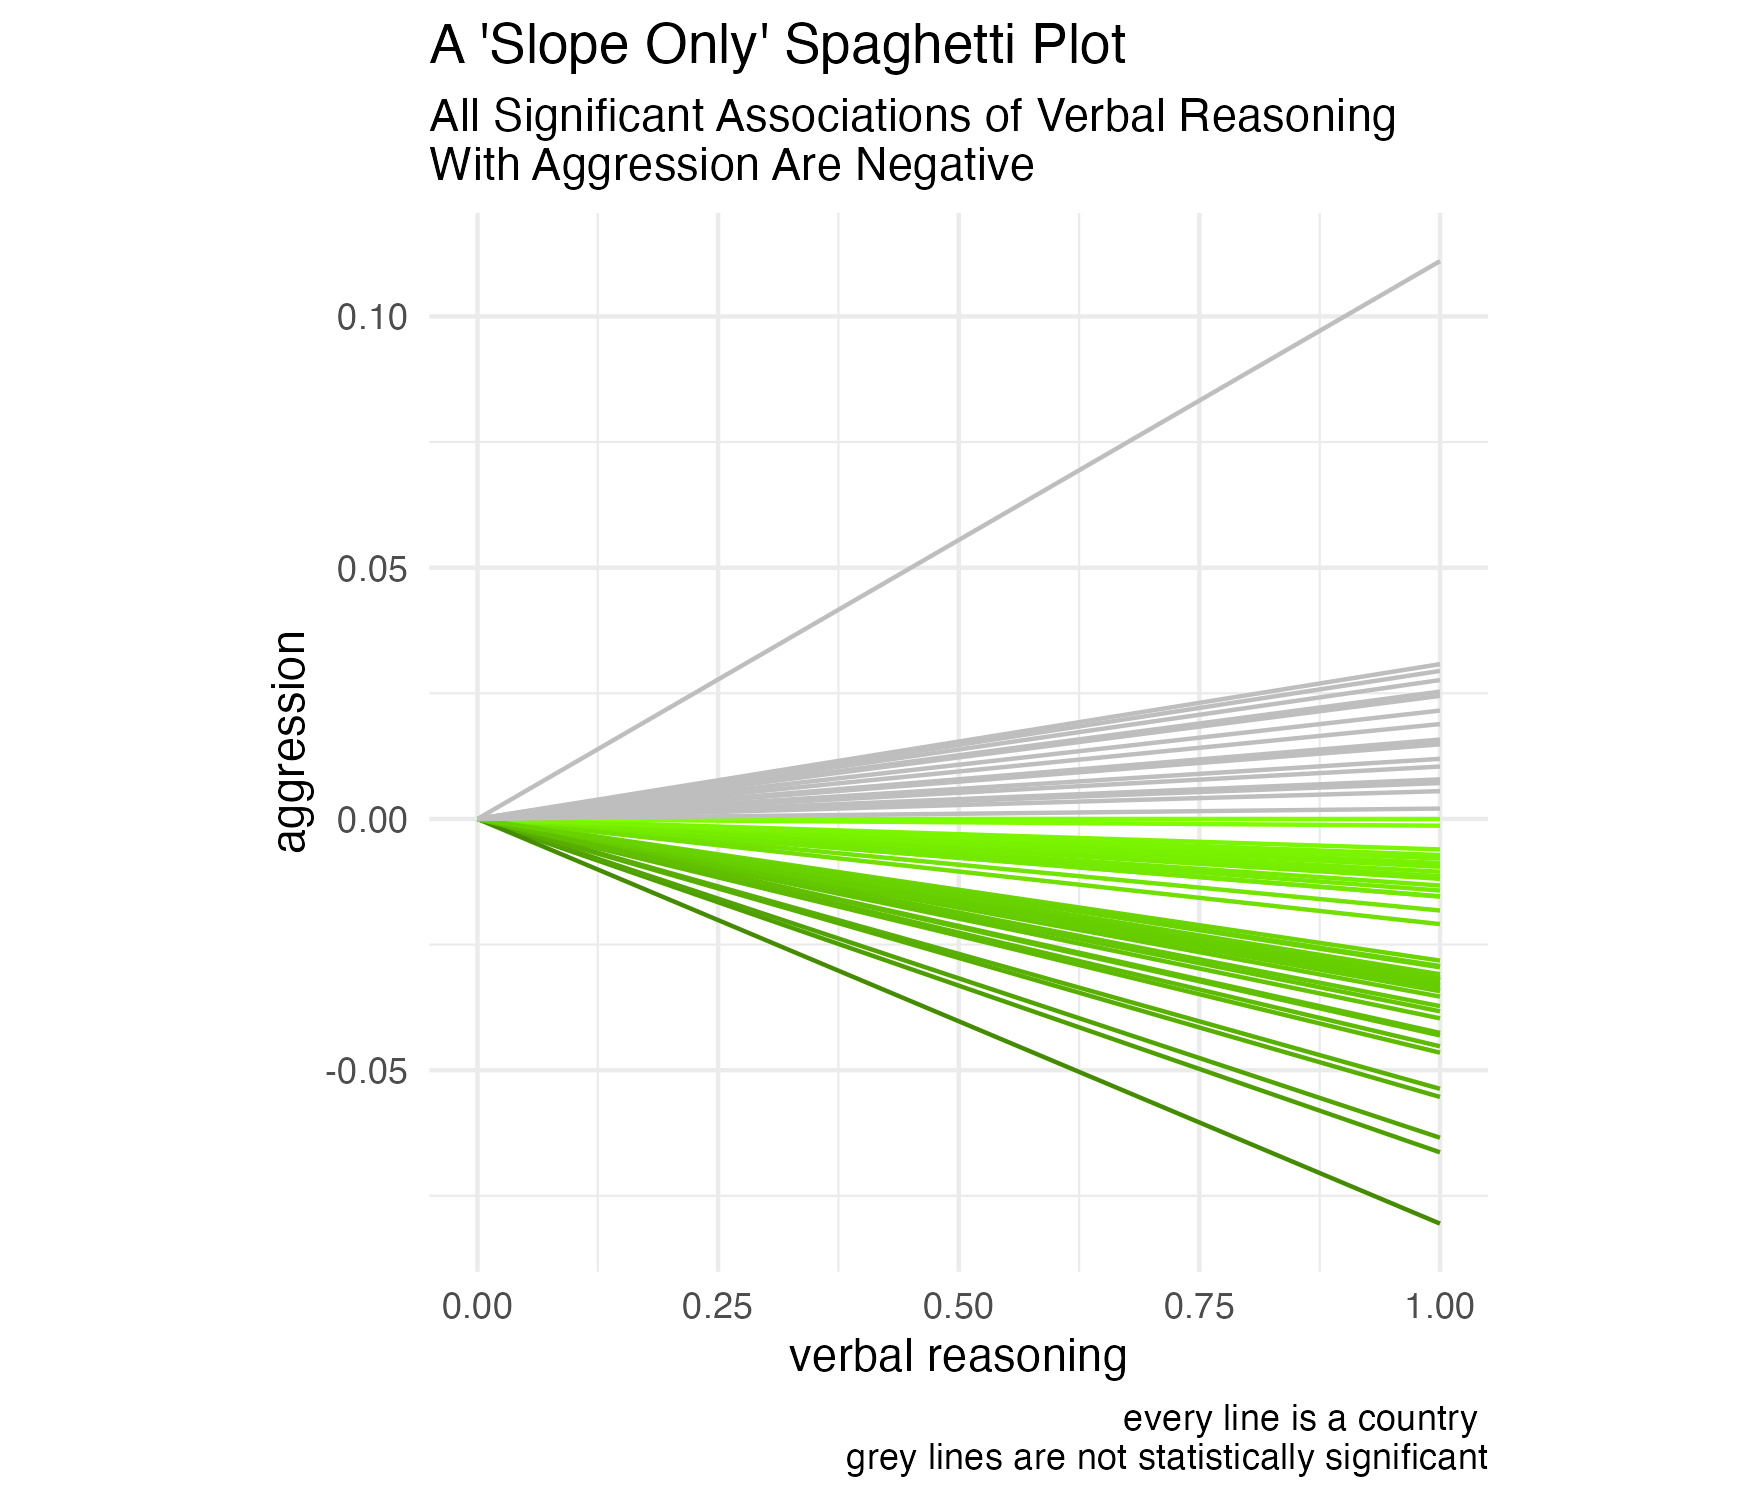
\includegraphics[keepaspectratio]{explain-spaghetti-plot.png}}

}

\caption{modified spaghetti plot}

\end{figure}%

\subsection{Quantifying Diversity and Commonality in the Relationship of
Parenting To Child
Outcomes}\label{quantifying-diversity-and-commonality-in-the-relationship-of-parenting-to-child-outcomes}

\begin{enumerate}
\def\labelenumi{\arabic{enumi}.}
\tightlist
\item
  {Regression slopes--when statistically significant--are all in the
  same direction}, and of at least somewhat similar magnitude.
\item
  The {actual values of the \(\text{var}(u_{kj})\) or
  \(\text{range}(u_{kj})\) are small}.
\end{enumerate}

\section{Wrapping It Up}\label{wrapping-it-up}

\subsection{To Summarize \ldots{}}\label{to-summarize}

\begin{itemize}
\tightlist
\item
  There is an {incredible diversity} across countries, especially
  LMIC's.
\item
  However, the {associations} of different forms of parental discipline
  are {surprisingly consistent}.

  \begin{itemize}
  \tightlist
  \item
    Explaining to children the difference between right and wrong has
    consistently {``good''} outcomes in terms of aggression.
  \item
    Spanking has consistently {``bad''} outcomes in terms of aggression.
  \item
    Shouting has consistently {``bad''} outcomes in terms of aggression.
  \item
    Name calling has consistently {``bad''} outcomes in terms of
    aggression.
  \end{itemize}
\end{itemize}

\subsection{Attempting a Visual
Summary\ldots{}}\label{attempting-a-visual-summary}

\begin{figure}[H]

{\centering 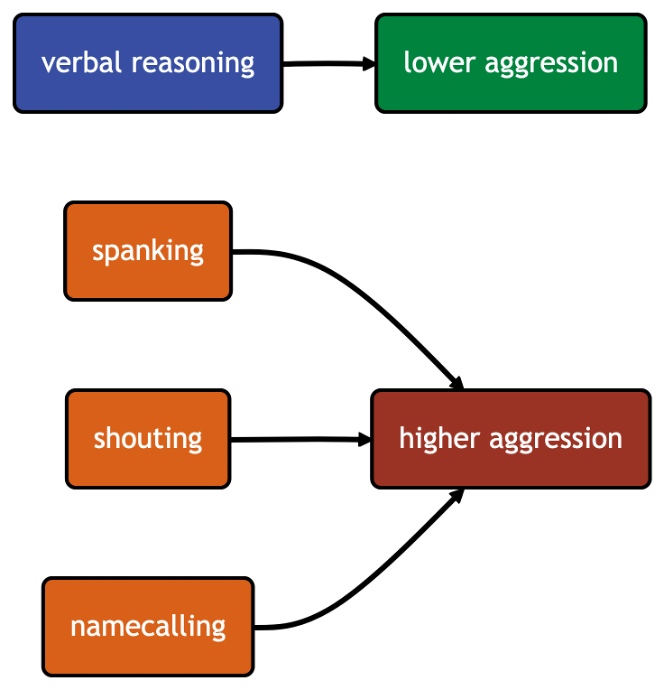
\includegraphics[width=0.5\linewidth,height=\textheight,keepaspectratio]{visual-summary-diagram.png}

}

\caption{a visual summary}

\end{figure}%

\subsection{Implications}\label{implications}

\begin{quote}
``My conception of the universal is that of a universal enriched by all
that is particular, a universal enriched by every particular: the
deepening and coexistence of all particulars.'' (Césaire, 1956)
\end{quote}

\begin{itemize}
\tightlist
\item
  Associations of parental discipline with child outcomes are {very
  consistent across countries}.
\item
  This {may be helpful} to international organizations (e.g.~UNICEF,
  WHO) that are developing programs or interventions that are to be
  applied in multiple cultural settings.
\item
  While cultural tailoring will always be necessary to some degree;
  {child development research can inform the foundations of widely
  applicable interventions}.
\end{itemize}

\begin{figure}[H]

{\centering \pandocbounded{
\includegraphics[keepaspectratio]{MICS.png}}

}

\caption{countries in MICS data}

\end{figure}%

\subsection{Discussion and Questions}\label{discussion-and-questions}

How might it be helpful to start thinking about possible {universality,
commonality, and similarity \ldots{}}

\ldots{} while keeping in mind \ldots{}

{\ldots{} our diversity, differences, and variation?}

\subsubsection{\texorpdfstring{\textbf{Other
Questions?}}{Other Questions?}}\label{other-questions}

\section*{References}\label{references-1}
\addcontentsline{toc}{section}{References}

\protect\phantomsection\label{refs}
\begin{CSLReferences}{1}{0}
\bibitem[\citeproctext]{ref-Antweiler2016}
Antweiler, C. (2016). \emph{Our common denominator: Human universals
revisited}. Berghahn.

\bibitem[\citeproctext]{ref-Barr2013}
Barr, D. J., Levy, R., Scheepers, C., \& Tily, H. J. (2013). Random
effects structure for confirmatory hypothesis testing: Keep it maximal.
\emph{Journal of Memory and Language}, \emph{68}(3), 255--278.
\url{https://doi.org/10.1016/j.jml.2012.11.001}

\bibitem[\citeproctext]{ref-Cesaire1956}
Césaire, A. (1956). Letter to {M}aurice {T}horez. \emph{Présence
Africaine.}

\bibitem[\citeproctext]{ref-Frank2018}
Frank, M. (2018). \emph{Mixed effects models: Is it time to go
{B}ayesian by default?}
\url{http://babieslearninglanguage.blogspot.com/2018/02/mixed-effects-models-is-it-time-to-go.html}

\bibitem[\citeproctext]{ref-Gershoff2016}
Gershoff, E. T., \& Grogan-Kaylor, A. (2016). Spanking and child
outcomes: Old controversies and new meta-analyses. \emph{Journal of
Family Psychology}, \emph{30}, 453--469.
\url{https://doi.org/10.1037/fam0000191}

\bibitem[\citeproctext]{ref-Hanel2019}
Hanel, P. H. P., Maio, G. R., \& Manstead, A. S. R. (2019). A new way to
look at the data: Similarities between groups of people are large and
important. \emph{Journal of Personality and Social Psychology},
\emph{116}, 541--562. \url{https://doi.org/10.1037/pspi0000154}

\bibitem[\citeproctext]{ref-Hunt-Hendrix2024}
Hunt-Hendrix, L., \& Taylor, A. (2024). \emph{Solidarity: The past,
present, and future of a world-changing idea}. Pantheon Books,.

\bibitem[\citeproctext]{ref-UNICEF2024fastfacts}
UNICEF. (2024a). \emph{FAST FACTS: Violence against children widespread,
affecting millions globally}.
\url{https://www.unicef.org/press-releases/fast-facts-violence-against-children-widespread-affecting-millions-globally}

\bibitem[\citeproctext]{ref-UNICEF2024notnewnormal}
UNICEF. (2024b). \emph{{``Not the new normal''} -- 2024 'one of the
worst years in UNICEF's history' for children in conflict}.
\url{https://www.unicef.org/press-releases/not-new-normal-2024-one-worst-years-unicefs-history-children-conflict}

\bibitem[\citeproctext]{ref-Ward2023}
Ward, K. P., Grogan-Kaylor, A. C., Ma, J., Pace, G., \& Lee, S. J.
(2023). Associations between 11 parental discipline behaviors and child
outcomes across 60 countries. \emph{BMJ Open}.
\url{https://doi.org/10.1136/bmjopen-2021-058439}

\end{CSLReferences}




\end{document}
